\documentclass{beamer}
\usetheme{Boadilla}

\newcommand\PRESENTATIONMODE[0]{signal command to allow beamer to work with the header file}

\newcommand\script[1]{}


%% Don't import the header multiple times

\ifdefined\HEADERIMPORTED
\else
\newcommand\HEADERIMPORTED[0]{This file is HEADERIMPORTED}
\usepackage{amssymb}

\usepackage{amsmath}
\usepackage[a4paper,includeheadfoot,margin=2.54cm]{geometry}

% For typesetting tree rules
\usepackage{mathpartir}

% For colouring code
\usepackage{xcolor}


\usepackage{array}   % for \newcolumntype macro
\usepackage{tikz-cd}
\usepackage{tabstackengine}
\usepackage{breqn}
\usepackage{stmaryrd}

\usepackage{framed}
\usepackage{listings}

\usepackage{amsthm}
%Theorems
\usepackage[utf8]{inputenc}
\usepackage[english]{babel}
\newtheorem{theorem}{Theorem}[section]
\newtheorem{corollary}{Corollary}[theorem]
\newtheorem{lemma}[theorem]{Lemma}
\newtheorem{property}[theorem]{Property}
\theoremstyle{definition}
\newtheorem{definition}{Definition}[section]

\usepackage{tikz}

\definecolor{grey}{rgb}{0.75, 0.75, 0.75}
\definecolor{DarkGreen}{rgb}{0.1, 0.6, 0.1}

\usetikzlibrary{shapes.geometric,fit}
\usetikzlibrary{arrows,automata,positioning}
\usetikzlibrary{decorations.pathreplacing,calc}



\setstackEOL{\cr}
\setstackgap{L}{\normalbaselineskip}

\newcommand\todo[1]{\textbf{TODO: #1}}
\newcommand\needsRef[1]{\textbf{Reference Needed: (#1)}}
\newcommand\fixLayout[1]{\textbf{Fix Layout: #1}}

\newcommand{\s}{\;}
\newcommand{\doin}[3]{\texttt{do}\s #1 \leftarrow #2 \s\texttt{in}\s #3\s}
\newcommand\apply[2]{#1\s#2}
\newcommand{\pifthenelse}[4]{\texttt{if}_{\textcolor{grey}{#1}}\s#2\s \texttt{then}\s #3 \s\texttt{else} \s#4\s}
\newcommand\ifthenelse[5]{\pifthenelse{#1, #2}{#3}{#4}{#5}}
\newcommand\const[1]{\texttt{C}^{\color{grey} #1}}
\newcommand\return[1]{\texttt{return} \s#1\s}


\newcommand\lam[3]{\lambda #1 \colon {\color{grey}#2}. #3\s}
\renewcommand\u[0]{\texttt{()}}
\newcommand{\U}[0]{\texttt{Unit}}
\renewcommand\t[0]{\texttt{true}}
\newcommand\f[0]{\texttt{false}}
\newcommand{\B}[0]{\texttt{Bool}}
\newcommand{\G}[0]{\Gamma}
\newcommand\D{\Delta}


% draw type relations
\newcommand{\typerelation}[3]{{\color{DarkGreen}#1} \vdash #2 \colon {\color{blue}#3}}
\newcommand\wellformed[2]{{\color{DarkGreen}#1}\vdash {\color{blue}#2}}
\newcommand\wellformedok[2]{\ok{{\color{DarkGreen}#1}\vdash {\color{blue} #2}}}



\newcommand{\gtyperelation}[2]{\typerelation{\G}{#1}{#2}}
 

\newcommand\treerulez[1]{\inferrule{ }{#1}}
\newcommand\treeruleI[2]{\inferrule{#1}{#2}}
\newcommand\treeruleII[3]{\inferrule{#1 \\ #2}{#3}}
\newcommand\treeruleIII[4]{\inferrule{#1 \\ #2 \\ #3}{#4}}
\newcommand\treeruleIV[5]{\inferrule{#1 \\ #2 \\ #3 \\ #4}{#5}}
\newcommand\treeruleV[6]{\inferrule{#1 \\ #2 \\ #3 \\ #4 \\ #5}{#6}}

\newcommand\ntreerulez[2]{(\text{#1})\inferrule{ }{#2}}
\newcommand\ntreeruleI[3]{(\text{#1})\inferrule{#2}{#3}}
\newcommand\ntreeruleII[4]{(\text{#1})\inferrule{#2 \\ #3}{#4}}
\newcommand\ntreeruleIII[5]{(\text{#1})\inferrule{#2 \\ #3 \\ #4}{#5}}
\newcommand\ntreeruleIV[6]{(\text{#1})\inferrule{#2 \\ #3 \\ #4 \\ #5}{#6}}
\newcommand\ntreeruleV[7]{(\text{#1})\inferrule{#2 \\ #3 \\ #4 \\ #5 \\ #6}{#7}}

\newcommand\condtreerulez[3]{(\text{#1})\inferrule{ }{#2}(\text{if } #3)}
\newcommand\condtreeruleI[4]{(\text{#1})\inferrule{#2}{#3}(\text{if } #4)}
\newcommand\condtreeruleII[5]{(\text{#1})\inferrule{#2 \\ #3}{#4}(\text{if } #5)}
\newcommand\condtreeruleIII[6]{(\text{#1})\inferrule{#2 \\ #3 \\ #4}{#5}(\text{if } #6)}
\newcommand\condtreeruleIV[7]{(\text{#1})\inferrule{#2 \\ #3 \\ #4 \\ #5}{#6}(\text{if } #7)}
\newcommand\condtreeruleV[8]{(\text{#1})\inferrule{ #2 \\ #3 \\ #4 \\ #5 \\ #6 }{#7}(\text{if } #8)}



\newcommand{\subtype}[0]{\leq\colon}
\newcommand\subeffect[0]{\leq}

\newcommand{\M}[2]{\texttt{M}_{#1}{#2}}

\newcommand\lamtype[3]{#1 \rightarrow \M{#2}{#3}}
\newcommand{\1}[0]{\texttt{1}}

\newcommand\e[0]{\epsilon}

\newcommand{\db}[1]{{\bf [\![}#1{\bf ]\!]}}
\newcommand{\deno}[1]{\db{#1}}
\newcommand\after\circ
\newcommand\term[1]{\left\langle\right\rangle_{#1}}

\newcommand\bindmu[0]{\mu}
\newcommand\point[1]{\eta_{#1}}
\newcommand\bind[3]{\bindmu_{#1, #2, #3}}

\newcommand\T[2]{T_{#1}{#2}}

\newcommand\pr[2]{\langle#1, #2\rangle}
\newcommand\finpr[2]{\langle #1\rangle_{#2}}

\newcommand\strengtht[0]{\texttt{t}}
% tensor strength Nat-tran
\newcommand\tstrength[3]{\strengtht_{#1, #2, #3}}

% Id morphism
\newcommand\Id[1]{\texttt{Id}_{#1}}

\newcommand\idg[0]{\Id{\G}}
% beta-eta equivalence
\newcommand\beequiv[0]{\approx}
% Substitutions
\newcommand\si{\sigma}

\newcommand{\sub}[1]{\left[#1\right]}
\newcommand{\ssub}[2]{\left[#2 / #1\right]}
\newcommand{\ssi}[0]{\sub{\si}}

% beta-eta equivalence relation
\newcommand{\berelation}[4]{\typerelation{#1}{#2 \beequiv #3}{#4}}
\newcommand{\gberelation}[3]{\gtyperelation{#1 \beequiv #2}{#3}}


% Shortcuts for denotational equality
\newcommand{\denoequality}[4]{\deno{\typerelation{#1}{#2}{#4}} = \deno{\typerelation{#1}{#3}{#4}}}
\newcommand{\gdenoequality}[3]{\denoequality{\G}{#1}{#2}{#3}}

% Shorthand for monad types
\newcommand\mea[0]{\M{\e}{A}}
\newcommand\meb[0]{\M{\e}{B}}
\newcommand\mec[0]{\M{\e}{C}}

\newcommand\tea[0]{\T{\e}{A}}
\newcommand\teb[0]{\T{\e}{B}}
\newcommand\tec[0]{\T{\e}{C}}


\newcommand\moa[0]{\M{\1}{A}}
\newcommand\mob[0]{\M{\1}{B}}
\newcommand\moc[0]{\M{\1}{C}}

\newcommand\toa[0]{\T{\1}{A}}
\newcommand\tob[0]{\T{\1}{B}}
\newcommand\toc[0]{\T{\1}{C}}

\newcommand\aeb[0]{\lamtype{A}{\e}{B}}

% Shorthand for Gammas
\newcommand{\gax}[0]{\G, x\colon A}
\newcommand{\gby}[0]{\G, y\colon B}

% reduction function
\newcommand{\reduce}[0]{reduce}



% Combinators for building delta-based tree proof terms
\newcommand{\deltavrule}[4]{
    \ntreeruleII{Subtype}{\treeruleI{\D}{\typerelation{#1}{#2}{#3}}}{#3 \subtype #4}{\typerelation{#1}{#2}{#4}}}

\newcommand{\deltavruleprime}[4]{
    \ntreeruleII{Subtype}{\treeruleI{\D'}{\typerelation{#1}{#2}{#3}}}{#3 \subtype #4}{\typerelation{#1}{#2}{#4}}}

\newcommand{\deltavruleprimeprime}[4]{
        \ntreeruleII{Subtype}{\treeruleI{\D'}{\typerelation{#1}{#2}{#3}}}{#3 \subtype #4}{\typerelation{#1}{#2}{#4}}}
    
\newcommand{\deltacrule}[6]{
            \ntreeruleII{Subeffect}{\treeruleI{\D}{\typerelation{#1}{#2}{\M{#3}{#4}}}}{\subeffecttree{#3}{#4}{#5}{#6}}{\typerelation{#1}{#2}{\M{#5}{#6}}}}
\newcommand{\deltacruleprime}[6]{
    \ntreeruleII{Subeffect}{\treeruleI{\D'}{\typerelation{#1}{#2}{\M{#3}{#4}}}}{
    \subeffecttree{#3}{#4}{#5}{#6}}{\typerelation{#1}{#2}{\M{#5}{#6}}}}
\newcommand{\deltacruleprimeprime}[6]{
    \ntreeruleII{Subtype}{\treeruleI{\D''}{\typerelation{#1}{#2}{\M{#3}{#4}}}}{
        \subeffecttree{#3}{#4}{#5}{#6}}{\typerelation{#1}{#2}{\M{#5}{#6}}}}
                            

\newcommand{\p}[0]{\pi_1}
\newcommand{\pp}[0]{\pi_2}

% short-hands for weakening
\newcommand{\wrel}[3]{#1 \colon {\color{blue}#2} \triangleright {\color {blue} #3}}
\newcommand{\ok}[1]{{\color{blue} #1} \texttt{ Ok}}
\renewcommand\i[0]{\iota}
\newcommand\w{\omega}
\newcommand\dom[1]{\texttt{dom}(#1)}
\newcommand\x{\times}


\newcommand\fev[1]{fev(#1)}
\newcommand\union[0]{\cup}


% Combinators to build tree proofs
\newcommand{\truleconst}[0]{\ntreeruleI{Const}{\ok{\G}}{\gtyperelation{\const{A}}{A}}}
\newcommand{\truleunit}[0]{\ntreeruleI{Unit}{\ok{\G}}{\typerelation{\G}{\u}{\U}}}
\newcommand{\truletrue}[0]{\ntreeruleI{True}{\ok{\G}}{\typerelation{\G}{\t}{\B}}}
\newcommand{\trulefalse}[0]{\ntreeruleI{False}{\ok{\G}}{\typerelation{\G}{\f}{\B}}}


\newcommand{\E}[0]{\mathbb{E}}
\renewcommand{\dot}{\cdot}
\newcommand{\gens}[0]{\colon\colon=}
\newcommand{\nil}[0]{\diamond}
\newcommand{\ground}[0]{\gamma}

% Terminal object of C
\newcommand{\terminal}[0]{\texttt{\1}}

% The category C
\newcommand{\C}[0]{\mathbb{C}}
\newcommand{\Cz}[0]{\C_0}
\newcommand\DC[0]{\mathbb{D}}

% The category of locally-small categories
\newcommand{\Cat}[0]{\texttt{Cat}}
% Sub-effect Nat-trans
\newcommand{\dse}[2]{\db{#1 \subeffect #2}}

\newcommand\app[0]{\texttt{app}}
\newcommand\cur[1]{\texttt{cur}(#1)}
\newcommand{\ifnt}[1]{\texttt{If}_{#1}}


\newcommand{\setto}{\colon=}
\newcommand{\fv}[1]{\texttt{fv}(#1)}

% shorthand for inserting text to equations
\newcommand\qt[1]{\quad\text{#1}}

% Co-product short-hands
\newcommand\inr[0]{\texttt{inr}}
\newcommand\inl[0]{\texttt{inl}}
    
\newcommand\fld[2]{\left[#1,#2\right]}
\newcommand{\diag}[1]{\delta_{#1}}
\newcommand{\twist}[2]{\tau_{#1, #2}}

\newcommand\ifMorph[3]{\app\after((\fld{\cur{#2\after\pp}}{\cur{#3\after\pp}}\after #1)\times \idg)\after \diag{\G}}


% Polymorphic short-hands
\newcommand\elam[2]{\Lambda #1. #2}
\newcommand{\eapp}[2]{#1\s#2}
\renewcommand{\a}[0]{\alpha}
\newcommand{\all}[2]{\forall #1. #2}
\renewcommand{\P}[0]{\Phi}

\renewcommand{\b}[0]{\beta}
\newcommand{\g}[0]{\gamma}
\renewcommand\d[0]{\delta}
\newcommand\oke[2]{\wellformedok{#1}{#2}}
\newcommand\etyperelation[4]{\typerelation{#1\mid#2}{#3}{#4}}
\newcommand{\gpetyperelation}[2]{\etyperelation{\P}{\G}{#1}{#2}}
\newcommand{\gppetyperelation}[2]{\etyperelation{\P'}{\G}{#1}{#2}}


\newcommand{\eberelation}[5]{\berelation{#1\mid#2}{#3}{#4}{#5}}
\newcommand{\gpeberelation}[3]{\berelation{\P\mid\G}{#1}{#2}{#3}}
\newcommand{\gppeberelation}[3]{\berelation{\P'\mid\G}{#1}{#2}{#3}}

\newcommand{\dotp}[0]{\dot_\P}
\newcommand{\fntype}[2]{#1\rightarrow #2}
\newcommand{\ab}[0]{\fntype{A}{B}}

\newcommand\wrelw[2]{\wrel{\w}{#1}{#2}}
\renewcommand\proof[0]{\paragraph{Proof:}}
\newcommand{\case}[1]{\paragraph{Case #1:}}
\newcommand{\subcase}[1]{\subparagraph{Case: #1}}
\newcommand\bi[0]{By inversion}

%pre-filled effect-weakening relations
\newcommand\ewrel[4]{\wellformed{#1}{\color{black}\wrel{#2}{#3}{#4}}}
\newcommand\pewrel[3]{\ewrel{\P}{#1}{#2}#3}
\newcommand\ppewrel[3]{\ewrel{\P'}{#1}{#2}#3}

\newcommand\subtypep[0]{\subtype_\P}
\newcommand\subtypepp[0]{\subtype_{\P'}}
\newcommand\subeffectp[0]{\subeffect_{\P}}
\newcommand\subeffectpp[0]{\subeffect_{\P'}}
\newcommand\subeffectn[0]{\subeffect_{n}}
\newcommand\subeffectz[0]{\subeffect_{0}}

\newcommand{\allI}[0]{\forall_I}
\newcommand{\allII}[0]{\forall_{I'}}
\newcommand\allIU[0]{\forall_{I\times U}}
\newcommand\type[0]{\texttt{Type}}
\newcommand\effect[0]{\texttt{Effect}}
\newcommand\ciw[0]{\C(I, W)}
\newcommand\ciu[0]{\C(I, U)}
\newcommand\ciuw[0]{\C(I\times U, W)}
\newcommand\cipw[0]{\C(I', W)}
\newcommand\cipu[0]{\C(I', U)}
\newcommand\ciuu[0]{\C(I\times U, U)}
\newcommand\cii[0]{\C(I', I)}
\newcommand\Eff[0]{\texttt{Eff}}
\newcommand\Mul[0]{\texttt{Mul}}
\newcommand\singleton[0]{\ast}
\renewcommand\star[0]{^*}
\renewcommand\bar[1]{\overline{#1}}

\newcommand\subtypeg[0]{\subtype_\g}
\newcommand\subtypepa[0]{\subtype_{\P, \a}}
\newcommand\subtypeppa[0]{\subtype_{\P', \a}}

\newcommand\subtypez[0]{\subtype_{0}}
\newcommand\subtypen[0]{\subtype_{n}}

\usepackage{scalerel,stackengine}
\stackMath
\renewcommand\widehat[1]{%
\savestack{\tmpbox}{\stretchto{%
  \scaleto{%
    \scalerel*[\widthof{\ensuremath{#1}}]{\kern.1pt\mathchar"0362\kern.1pt}%
    {\rule{0ex}{\textheight}}%WIDTH-LIMITED CIRCUMFLEX
  }{\textheight}% 
}{2.4ex}}%
\stackon[-6.9pt]{#1}{\tmpbox}%
}
\parskip 1ex

\newcommand\pstar[0]{\p\star}

\newcommand\edeltavrule[5]{\deltavrule{#1 \mid #2}{#3}{#4}{#5}}

\newcommand\subeffecttreep[4]{\ntreeruleII{Effect}{
    #1\subeffectp #3}{#2 \subtypep #4
}{\M{#1}{
    #2
}\subtypep\M{#3}{#4}}}
\newcommand\subeffecttree[4]{\ntreeruleII{Effect}{
    #1\subeffect #3}{#2 \subtype #4
}{\M{#1}{
    #2
}\subtype\M{#3}{#4}}}


\newcommand{\edeltavruleprime}[5]{
        \deltavruleprime{#1\mid #2}{#3}{#4}{#5}}
    
\newcommand{\edeltavruleprimeprime}[5]{
        \deltavruleprimeprime{#1\mid #2}{#3}{#4}{#5}}
    
\newcommand{\edeltacrule}[6]{
            \ntreeruleII{Subtype}{
                \treeruleI{
                    \D
                }{
                    \typerelation{\P\mid#1}{#2}{\M{#3}{#4}}
                }
            }{
                \ntreeruleII{Effect}{
                    #4 \subtypep #6
                    }{
                         #3 \subeffectp #5
                }{
                    \M{#3}{#4}\subtypep{\M{#5}{#6}}
                }
            }{
                \typerelation{\P\mid #1}{#2}{\M{#5}{#6}}
            }
        }
        

        \newcommand{\edeltacruleprime}[6]{
            \ntreeruleII{Subtype}{
                \treeruleI{
                    \D'
                }{
                    \typerelation{\P\mid #1}{#2}{\M{#3}{#4}}
                }
            }{
                \ntreeruleII{Effect}{
                    #4 \subtypep #6
                }{#3 \subeffectp #5
                }{
                    \M{#3}{#4}\subtypep{\M{#5}{#6}}
                }
            }{
                \typerelation{\P\mid #1}{#2}{\M{#5}{#6}}
            }
        }
                   

        \newcommand{\edeltacruleprimeprime}[6]{
            \ntreeruleII{Subtype}{
                \treeruleI{
                    \D''
                }{
                    \typerelation{\P\mid #1}{#2}{\M{#3}{#4}}
                }
            }{
                \ntreeruleII{Effect}{
                    #4 \subtypep #6
                    }{ #3 \subeffectp #5
                }{
                    \M{#3}{#4}\subtypep{\M{#5}{#6}}
                }
            }{
                \typerelation{\P\mid #1}{#2}{\M{#5}{#6}}
            }
        }

        \newcommand\obj[0]{\texttt{obj }}


        \newcommand{\Tz}[2]{\texttt{T}^0_{#1}#2}
        \newcommand{\Tn}[2]{\texttt{T}^n_{#1}#2}
        \newcommand{\Tm}[2]{\texttt{T}^m_{#1}#2}
        
        \newcommand{\pointz}[1]{\point{#1}^0}
        \newcommand{\pointn}[1]{\point{#1}^n}
        \newcommand{\pointm}[1]{\point{#1}^m}
        
        \newcommand{\bindz}[3]{\bind{#1}{#2}{#3}^0}
        \newcommand{\bindn}[3]{\bind{#1}{#2}{#3}^n}
        \newcommand{\bindm}[3]{\bind{#1}{#2}{#3}^m}
        
        \newcommand\tstrengthz[3]{\tstrength{#1}{#2}{#3}^0}
        \newcommand\tstrengthn[3]{\tstrength{#1}{#2}{#3}^n}
        \newcommand\tstrengthm[3]{\tstrength{#1}{#2}{#3}^m}
        
        \newcommand\set[0]{\texttt{Set}}
        \newcommand\cccat[0]{\textit{CCCat}}

        \newcommand\ev[0]{\vec{\e}}
        \newcommand\emv[0]{\vec{\e_m}}
        \newcommand\env[0]{\vec{\e_n}}
        
        \newcommand\subeffectm[0]{\subeffect_m}
        
        \newcommand\dsem[2]{\db{#1 \subeffectm #2}}
        \newcommand\dsen[2]{\db{#1 \subeffectn #2}}
        \newcommand\dsez[2]{\db{#1 \subeffectz #2}}
        \newcommand\dsep[2]{\db{#1 \subeffectp #2}}
        \newcommand\dsepp[2]{\db{#1 \subeffectpp #2}}
        
        \newcommand\allEn[0]{\forall_{E^n}}
        \newcommand\allEm[0]{\forall_{E^m}}
        
        \newcommand\counit[1]{\boldsymbol{\epsilon}_{#1}}
        \newcommand\unit[1]{\boldsymbol{\eta}_{#1}}
\fi

\title{A Denotational Semantics for Polymorphic Effect Systems}
\subtitle{Part III Project}
\author{Alexander Taylor, at736}
\institute{University of Cambridge}
\date{\today}

\newcommand\comment[1]{
    %
}


\comment{
How to give a scientific talk
- Most of the audience cannot refer to thing's you've alreay selectfont
- Can't ask qs (3-4 qs max)
- therefore, lapses of attention damage comprehension
- therefore talk define about managing attention

    - talk too hard/easy
    - motive unclear

- managing attention with narrative
    - stories + raise further questions
    - only simple narrative needed 
    - for 20 min talk  
        - 6 min motivation
        - 3 min contributions + key ideas
        - 9 mins of explanation
        - 2 mins conclusion

    - motivation
        - Top down: here is a problem, how do we solve it?
            - start with a problem, obvious that a solution is needed to audience
            - motivate search for solution
            - danger 
                - fail to clearly articulate the problem 
                - take too long to explain the problem
        - bottom up: we have observations, which raise questions
            - interesting observations
            - surprising connections between them
            - motivates the search for an explanation

            - dangers
                - boring observatiosn
                - connection boring to non-experts

    The Goal
        - Give your approach to the problem
        - identify one key idea of your solution
            - not zero
                - need to explain to something new
                - doesn't answer problem
            - not n+2
                - many papers require several innovations
                - find a unified way to describe this as one idea
                - otherwise the audience will be confused
    divide and conquer
        - divide the explanation into segment
        - treat each segment as mini talk  
            - motivation, idea, explanantion, conclusion
        - remind audience of what you did and why 
}


\begin{document}

\begin{frame}
    \titlepage
\end{frame}

\begin{frame}[fragile]{Motivating Polymorphic Effect Analysis}    

\begin{verbatim}
def logAction(
    action: Unit => String
): Unit {
    log.info(action())
}  
\end{verbatim}

\begin{verbatim}
logAction(() => FireMissiles(); "Launched Missiles)

logAction(() => throwError("My Error"))

logAction(() => readEnvironmentVariables)
\end{verbatim}

    \script{
        - Imagine you're a compiler trying to analyse the side effects of this \texttt{doAction} function here.

        - You're not having the best of times
        - it's used three times with three different side effect - one's irrevocable - you can't speculatively execute it, one alters control flow, and the last accesses immutable state so you can do all sorts of optimisations.
        
        - Using some simple  analysis, you can create three separate instantiations of the function to analyse, so it's not too difficult in this case.
        - However in programs with higher order functions, creating these separate instantiations is undecidable in general

        - With a polymorphic effect system, it becomes a bit easier to analyse programs like this. But how do you know that your tools and optimisations are sound?
    }
\end{frame}

\begin{frame}{What is denotational Semantics? }
    \begin{itemize}
        \item A mapping $\deno{-}: \text{Language Structure} \rightarrow \text{Mathematical Structure}$
        \item In particular want to define $\deno{\gtyperelation{t}{A}}$
        \item Needs to be \textit{compositional}, \textit{sound}
        \item And \textit{adequate} for our needs
    \end{itemize}

    \script{
        - Denotational semantics is where we create a mapping between program terms and an abstract mathematical structure.
        - We want this to be compositional - meaning that each term's denotation is defined in terms of its subterms 
        - It should also be sound, meaning that equivalent program terms up-for, for example, beta-eta reduction, have equal denotations.
        - we also want it to be adequate - if two terms have equal denotations, then that should mean something useful about the relation of the two terms (e.g. can replace one by the other, etc)
    }
\end{frame}

\begin{frame}{Denotational Semantics using Category Theory}
    \begin{itemize}
        \item Interested in: Objects, Morphisms, and Functors
        \item $\deno{A}, \deno{\G} \in\obj\C$
        \item $\deno{\gtyperelation{t}{A}}: \deno{\G}\rightarrow \deno{A}$
    \end{itemize}


    \script{
        - In part II, we used domains to handle the semantics of non-termination. Lurking beneath this notion is the idea that we can use category theoretic structure to construct our denotations.

        - Here we map types and type environments to objects in a particular category, and correctly typed terms to morphisms (arrows) in the category.

        - One more structure we need is a functor - a map of objects to objects and morphisms to morphisms that preserves composition of terms.
    }
\end{frame}

\begin{frame}{Language features (1) - Lambda Calculus}

        A cartesian closed category (CCC) consists of:
        \begin{itemize}
            \item Products $A\times B$ - models tuples
            \item A terminal object $\1$ - models the \U\texttt{  }type
            \item Exponential objects $B^A$ - models functions as first-class objects
        \end{itemize}

        \script{
            Now let's look at what category theoretic structure you need to model different language features.
            
            - For lambda calculus style languages, you need at least a cartesian closed category.

            - In terms of the category of sets, this gives you sets of pairs of objects, sets of functions, and the single element set.

            - These are used to model pairs, lambda terms, giving us higher order functions, and the terminal, single element set allows us to interpret the unit type and ground terms.
        }
\end{frame}

\begin{frame}{Language features (2.A) - Monads}
        A (strong) monad consists of:
        \begin{itemize}
            \item A functor $\T{}{}: \C\rightarrow \C$
            \item Join and Unit natural transformations
            \begin{itemize}
                \item  $\bindmu_{A}: \T{}{\T{}{A}}\rightarrow \T{}{A}$
                \item $\point{A}: A\rightarrow \T{}{A}$
            \end{itemize}
            \item Tensor strength natural transformation $\strengtht_{A, B}: A\times\T{}{B}\rightarrow \T{}{(A\times B)}$
        \end{itemize}
        
        \script{
            - To handle effectful computations in a pure language like haskell, you need to use something called a monad.

            - This actually comes from when Moggi first discovered how to model effectful programs.
            - You need this structure of a functor from your category to itself, together with some natural transformation operations for creating and composing effectful operations.
            - If you squint a bit, they even look like the programming language monad definition.

            - An issue with haskell is that each monad only gives you one effect. If you want a program that does IO, contains state, has exceptions, and does non-determinism, you end up with a stack of monads.
            - This is still imprecise for meaningful analysis
        }


\end{frame}

\begin{frame}{Language features (2.B) - Graded Monads}
    A (strong) graded monad consists of:
        \begin{itemize}
            \item An indexed functor $\T{\e}{}: \C\rightarrow \C$
            \item Indexed Join and Unit natural transformations
            \begin{itemize}
                \item  $\bind{\e_1}{\e_2}{A}: \T{\e_1}{\T{\e_2}{A}}\rightarrow \T{\e_1\dot \e_2}{A}$\
                \item $\point{A}: A\rightarrow \T{\1}{A}$
            \end{itemize}
            \item Tensor strength natural transformation $\tstrength{\e}{A}{B}: A\times\T{\e}{B}\rightarrow \T{\e}{(A\times B)}$
        \end{itemize}

        \script{
            - A solution is a graded monad.
            - We now have one functor, indexed by a monoid of effect symbols. The rules and morphisms stay the same but are now also indexed. 

        }    
\end{frame}

\begin{frame}{Language Features (3.A) - If-Expressions}
    - If expression example
    - Co-product diagram

    \begin{itemize}
        \item $\pifthenelse{A}{b}{t}{f}$
        \item If expressions modelled by co-products
        \item 
        \begin{tikzcd}[ampersand replacement=\&]
            \&  A   \& \\
            \G \arrow{ur}{t} \arrow [r, "\inl"] \&   (\G + \G) \arrow{u}{[t, f]}  \& \arrow{l}[swap]{\inr} \arrow{ul}[swap]{f} \G\\
        \end{tikzcd}
    \end{itemize}
    


    \script{
        - Finally, we may want to add if expressions to our language. 
        - This can be fairly easily be done using co-products (the generalisation of what disjoint unions on sets are)
     }
\end{frame}

\begin{frame}[fragile]{Language Features 3.B - An Issue}
    Consider this:

\begin{verbatim}
    if (UserConfirms) then Save() else pass;
\end{verbatim}

\begin{itemize}
    \item Branches have different effects
    \item So have different types!
    \item This doesn't type correctly
\end{itemize}

\script{        
    - But leads to an issue when effects are involved. Both branches of the expression need to have the same type, but we might want to write programs where one side has a different effect.
}

\end{frame}

\begin{frame}{Language Features 3.C - Subtyping}
    $$\ntreeruleII{Subtype}{\gtyperelation{t}{A}}{A \subtype B}{\gtyperelation{t}{B}}$$

    \begin{itemize}
        \item This needs a denotation
        \item So introduce $\deno{A\subtype B}$
        \item $\deno{\gtyperelation{t}{B}} = \deno{A\subtype B}\after \deno{\gtyperelation{t}{A}}$
    \end{itemize}

    \script{
        - To allow more programs to type correctly, we need to introduce subtyping and appropriate morphisms to handle this.
    }
\end{frame}

\begin{frame}{An Effectful Language}
    \begin{align*}
        v ::= & \const{A} \mid x\mid \t \mid\f \mid\u\mid\lam{x}{A}{v}\mid\apply{v_1}{v_2}\mid\return{v}\\
        & \mid\doin{x}{v_1}{v_2}\mid\pifthenelse{A}{v}{v_1}{v_2} 
    \end{align*}
    
    \begin{align*}
        A, B, C ::= \g\mid \ab \mid\mea
    \end{align*}

    \[
        \ntreeruleI{Return}{\gtyperelation{v}{A}}{\gtyperelation{\return{v}}{\moa}}
    \quad
    \ntreeruleII{Apply}{\gtyperelation{v_1}{\ab}}{\gtyperelation{v_2}{A}}{\gtyperelation{\apply{v_1}{v_2}}{B}}
    \]

    \script{
        - Let's now describe a simple effectful, lambda-calculus-based, language, EC.
        - It has an explicit graded monad, subtyping, if-statements
    }
\end{frame}

\begin{frame}{Semantics of EC}
    \begin{itemize}
        \item Can build a model of EC when we have
        \begin{itemize}
            \item CCC
            \item Co-product
            \item Strong Graded Monad
            \item Subtyping morphisms
        \end{itemize}
        \item We'll call this an S-category
    \end{itemize}
    
    \[
        \scalebox{.8}{$
        \ntreeruleI{Return}{f = \deno{\gtyperelation{v}{A}}}{\deno{\gtyperelation{\return{v}}{\moa}} = \point{A} \after f}
        \quad
        \ntreeruleI{Fn}{f = \deno{\typerelation{\gax}{v}{B}} : \G \times A \rightarrow B}{\deno{\gtyperelation{\lam{x}{A}{v}}{\ab}} = \cur{f} : \G \rightarrow B^A}
        $}
    \]

    \script{
        - As described, all of the language features can be modelled in a cartesian closed category with a graded monad, a coproduct, and subtyping morphisms.

        - Known as an S-Category

        - Here's an example, if we have the denotation of an expression here, we can get the denotation of using it as a pure computation by postcomposing with the unit of the graded monad.

    }
\end{frame}

\begin{frame}[fragile]{An Ugly Example}

    \begin{lstlisting}[
        mathescape,
        columns=fullflexible,
        basicstyle=\fontfamily{lmvtt}\selectfont,
      ]
let $twiceIO$ = $\lambda$ $action$: $\M{\texttt{IO}}{\U}$. (
    do $\_$ $\texttt{<-}$ $action$ in $action$
)

let $twiceState$ = $\lambda$ $action$: $\M{\texttt{State}}{\U}$. (
    do $\_$ $\texttt{<-}$ $action$ in $action$
)

do $\_$ $\texttt{<-}$ $twiceState$(increment) in $twiceIO$(writeLog)
    \end{lstlisting}
    \script{
        - Here's a program that's quite ugly with lots of code reuse, since we explicitly state types in the expressions. 
        - we end up with two instantiations of the same function - more work for the compiler
    }
\end{frame}

\begin{frame}{Let's Add Polymorphism}
   
\begin{align*}
    v::=\text{..}\mid\elam{\a}{v}\mid\eapp{v}{\e}
\end{align*}

\begin{align*}
    A, B, C::=\text{...}\mid \all{\a}{A}
\end{align*}

\begin{align*}
    \e ::= e \mid \a \mid \e\dot\e
\end{align*}

    \[
        \ntreeruleI{Effect-Gen}{\etyperelation{\P,\a}{\G}{v}{A}}{\gpetyperelation{\elam{\a}{v}}{\all{\a}{A}}}
        \quad
        \ntreeruleII{Effect-Spec}{\gpetyperelation{v}{\all{\a}A}}{\wellformed{\P}{\e}}{\gpetyperelation{\eapp{v}{\e}}{A\ssub{\a}{\e}}}    
    \]
    \script{
        - Let's now add some polymorphism syntax to EC.
        - This gives us the polymorphic effect calculus.
        - Notice now that in our type rules, we now have an effect-variable environment. Important later
    }
\end{frame}

\begin{frame}[fragile]{An Ugly Example - With a Makeover}
    \begin{lstlisting}[
        mathescape,
        columns=fullflexible,
        basicstyle=\fontfamily{lmvtt}\selectfont,
      ]
let $twice$ = $\Lambda$ $eff$.(
    $\lambda$ $action$: $\M{eff}{\U}$. (
        do $\_$ $\texttt{<-}$ $action$ in $action$
    )
)

do $\_$ $\texttt{<-}$ ($twice$ State increment) in ($twice$ IO writeLog)
    \end{lstlisting}
    \script{
        - We've now added polymorphism, which makes our ugly program more concise.
        - We can reuse this function
    }
\end{frame}

\begin{frame}{How do we Model the Semantics of a Polymorphic Language?}

    \begin{itemize}
        \item For a fixed effect variable environment $\P$ and terms with no polymorphic sub-terms, we have EC
        \item Effect-variable environments of length $n$ are isomorphic by $\a$-equivalence
    \end{itemize}
    
    

    \script{
        - If we fix the effect-variable environment, and disallow polymorphic terms, then PEC terms become EC terms for a particular instantiation.
        - We already know how to build models for PEC
        -It's also the case that effect-variable environments can type the same set of relations, upto alpha equivalence.
        - So there is a countable set of these EC instantiations
    }
\end{frame}

\begin{frame}{How do we Model the Semantics of a Polymorphic Language?}
    - Stack of S-categories and their morphisms

    - type rule for generalisation
    - "Need functors"

\script{
    - So we can imagine a stack of these S-Categories, called fibres
    - In order to model polymorphism, we need to have ways of moving morphisms between these fibres - we need functors
}
\end{frame}

\begin{frame}{Base Category}
    - We need a way of reasoning about effect-variable environment categorically

    - We can model effects and environments in new category.

    - Objects: $\1$, $U$, $U^n$ (write I for $U^n$)
    - Morphisms: $\deno{e}: \1\rightarrow U$
    - Monoidal operator $\Mul: \ciu\times\ciu\rightarrow\ciu$
    - Can represent each effect environment as an object $I$, and common transformations between environments, such as weakening and substitutions, are morphisms between effect environments.

    \script{
        - So we need a way of reasoning about the transformations of effect-variable environments in a category theoretic manner
        - To do this, we need a base category, containing a terminal object, an object $U$ representing the kind of effects, and finite products on $U$ 
        - $U^n$ represents the effect-variable environment of length $n$. We'll now use $I$ to indicate this.
        
        - Since all the ground effects have morphisms in this category, we can construct morphisms for substitutions and weakenings of the effect environment.
    }
\end{frame}

\begin{frame}{Indexed Category}

    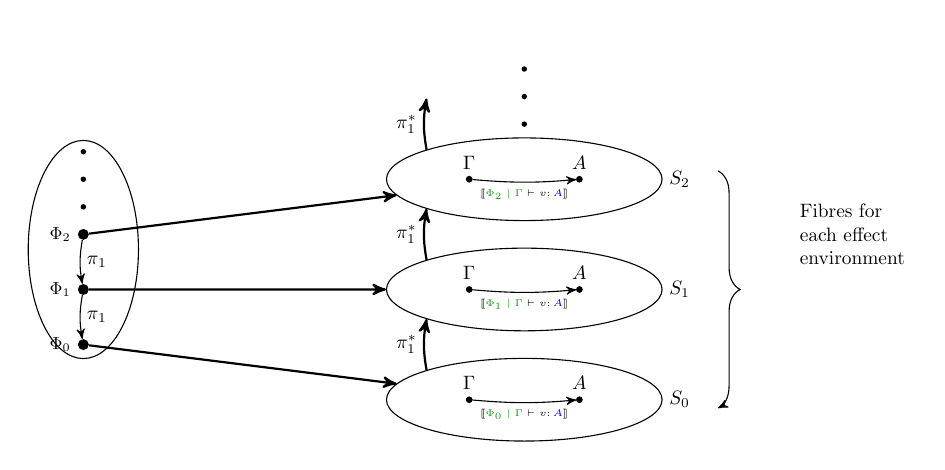
\begin{tikzpicture}[->,>=stealth', scale=0.7, every node/.style={scale=0.7}]
        % Draw the env objects
        \foreach \y[count=\c,evaluate={\yi=int(\c-1)}] in {3, 4, 5}{
            \node[fill,circle,inner sep=2pt,label=left:{\small $\P_\yi$}] (d\yi) at (0,\y) {};
        }

        % draw the ... above the env objects
        \foreach \y[count=\c,evaluate={\yi=int(\c-1)}] in {5.5, 6, 6.5}{
            \node[fill, circle, inner sep=1pt] (dd\yi) at (0,\y){};
        }
        % Draw the index category
        \node[fit=(d0) (d1) (d2) (dd0) (dd1) (dd2),ellipse,draw,minimum width=2cm] {};

        %draw the s-category stack
        \foreach \y[count=\c,evaluate={\yi=int(\c-1)}] in {2, 4, 6}{
            \node[circle, draw, inner sep=1pt, fill, label=above:{$\G$}] (g\yi) at (7,\y){};
            \node[circle, draw, inner sep=1pt, fill, label=above:{$A$}] (a\yi) at (9,\y){};
            \draw[->](g\yi) to[bend right=5] node[below]{\tiny $\deno{\etyperelation{\P_\yi}{\G}{v}{A}}$} (a\yi);
            \node[ellipse, draw, minimum width=5cm, minimum height=15mm,label=right:$S_\yi$] (s\yi) at (8,\y){};
        }

        % Hidden ellipse to draw functors to
        \node[ellipse, minimum width=5cm, minimum height=15mm] (s3) at (8,8){};

        %Draw the ... for the s-category stack
        \foreach \y[count=\c,evaluate={\yi=int(\c-1)}] in {7, 7.5, 8}{
            \node[fill, circle, inner sep=1pt] (p\yi) at (8, \y){};
        }

        % Draw index arrows
        \foreach \i in {0, 1, 2}{
            \draw[->, thick] (d\i) to (s\i);
        }

        % draw the re-indexing functors

        \foreach \source[count=\dest] in {0, 1, 2}{
            \draw[->, thick](s\source.north west) to[bend left=10] node[left]{$\pstar$} (s\dest.south west);
        }

        % Draw the quantification functors
        %\foreach \dest[count=\source] in {0, 1, 2}{
        %    \draw[->, thick] 
        %    (s\source.south east) to[bend left=10] node[right]{$\forall_{\P_\dest}$} (s\dest.north east);
        %}

        % Draw the internal morphisms in base category
        \foreach \dest[count=\source] in {0, 1}{
            \draw[->]
            (d\source) to[bend right=10] node[right]{$\p$} (d\dest);
        }

        %Draw the bracket

        \draw [decoration={brace,amplitude=8pt},decorate] ($(s2)+(10em,1ex)$) -- ($(s0)+(10em,-1ex)$);
        \node[text width=20mm] (Label) at (14,5){Fibres for each effect environment};
    \end{tikzpicture}


    \script{
        - So now we can construct this structure
        - called an index category
        - We have a functor mapping each object representing an effect-variable environment to the relevant S-category fibre.
        - Also contravariantly, meaning the direction of the morphism changes, maps morphisms in the base category to re-indexing functors between the relevant fibres.
        - So now we can perform substitutions and weakenings on the effect environment and get the right behaviour on the semantics of the EC instantiation
    }
    
\end{frame}

\begin{frame}{Quantification}
    \begin{itemize}
        \item What about effect-generalisation?
        \item $\ntreeruleI{Effect-Gen}{\etyperelation{\P,\a}{\G}{v}{A}}{\etyperelation{\P}{\G}{\elam{\a}{v}}{\all{\a}{A}}}$
        \item Need to map $\deno{\etyperelation{\P,\a}{\G}{v}{A}}$ to $\deno{\etyperelation{\P}{\G}{\elam{\a}{v}}{\all{\a}{A}}}$
        \item For specialisation to work, needs: $\pstar\dashv\allI$
    \end{itemize}


    
    \script{
        - We now need to think about the polymorphic terms
        - For quantification, we need another functor, $\allI$ which maps a type rule with an extra effect variable to one quantified over that variable
        - In order for specialisation to work, this quantification functor needs to be a right adjoint to the opposite operation of weakening the effect environment
        - Adjunction of functors is essentially a weaker version of an isomorphism of the categories they're between.
        - Going out on one functor and coming back on the other isn't quite the same as the identity, but it has a well defined action.
    }

\end{frame}
    
\begin{frame}{Instantiating a Model (1)}

        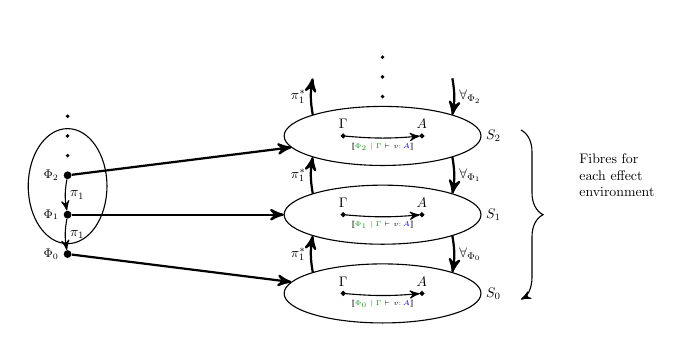
\begin{tikzpicture}[->,>=stealth', scale=0.5, every node/.style={scale=0.5}]
            % Draw the env objects
            \foreach \y[count=\c,evaluate={\yi=int(\c-1)}] in {3, 4, 5}{
                \node[fill,circle,inner sep=2pt,label=left:{\small $\P_\yi$}] (d\yi) at (0,\y) {};
            }
    
            % draw the ... above the env objects
            \foreach \y[count=\c,evaluate={\yi=int(\c-1)}] in {5.5, 6, 6.5}{
                \node[fill, circle, inner sep=1pt] (dd\yi) at (0,\y){};
            }
            % Draw the index category
            \node[fit=(d0) (d1) (d2) (dd0) (dd1) (dd2),ellipse,draw,minimum width=2cm] {};
    
            %draw the s-category stack
            \foreach \y[count=\c,evaluate={\yi=int(\c-1)}] in {2, 4, 6}{
                \node[circle, draw, inner sep=1pt, fill, label=above:{$\G$}] (g\yi) at (7,\y){};
                \node[circle, draw, inner sep=1pt, fill, label=above:{$A$}] (a\yi) at (9,\y){};
                \draw[->](g\yi) to[bend right=5] node[below]{\tiny $\deno{\etyperelation{\P_\yi}{\G}{v}{A}}$} (a\yi);
                \node[ellipse, draw, minimum width=5cm, minimum height=15mm,label=right:$S_\yi$] (s\yi) at (8,\y){};
            }
    
            % Hidden ellipse to draw functors to
            \node[ellipse, minimum width=5cm, minimum height=15mm] (s3) at (8,8){};
    
            %Draw the ... for the s-category stack
            \foreach \y[count=\c,evaluate={\yi=int(\c-1)}] in {7, 7.5, 8}{
                \node[fill, circle, inner sep=1pt] (p\yi) at (8, \y){};
            }
    
            % Draw index arrows
            \foreach \i in {0, 1, 2}{
                \draw[->, thick] (d\i) to (s\i);
            }
    
            % draw the re-indexing functors
    
            \foreach \source[count=\dest] in {0, 1, 2}{
                \draw[->, thick](s\source.north west) to[bend left=10] node[left]{$\pstar$} (s\dest.south west);
            }
    
            % Draw the quantification functors
            \foreach \dest[count=\source] in {0, 1, 2}{
                \draw[->, thick] 
                (s\source.south east) to[bend left=10] node[right]{$\forall_{\P_\dest}$} (s\dest.north east);
            }
    
            % Draw the internal morphisms in base category
            \foreach \dest[count=\source] in {0, 1}{
                \draw[->]
                (d\source) to[bend right=10] node[right]{$\p$} (d\dest);
            }
    
            %Draw the bracket
    
            \draw [decoration={brace,amplitude=8pt},decorate] ($(s2)+(10em,1ex)$) -- ($(s0)+(10em,-1ex)$);
            \node[text width=20mm] (Label) at (14,5){Fibres for each effect environment};
        \end{tikzpicture}

    \begin{itemize}
        \item Can we actually instantiate a category with the required structure? 
        \item Starting point a model of EC in $\set$
    \end{itemize}
    
    \script{
        - So far, we've only said what structures are required to model PEC.
        - Haven't shown that there actually exists an indexed category with the required properties
        - so let's do that
        - It's fairly well known that you can instantiate models of languages with the same features as EC in the category of sets and functions
        - We want to extend one of these models into one for PEC
    }
\end{frame}

\begin{frame}{Instantiating a Model (2) - Base Category}
\begin{itemize}
    \item Use $\Eff$ - category of monotone functions of tuples of ground effects to ground effects
    \item $\deno{\typerelation{\nil,\a, \b}{\b\dot(\a\dot\texttt{IO})}{\effect}} = (e_1, e_2)\mapsto e_2\dot(e_1\dot\texttt{IO})$
    \item $\Mul(f, g)\ev = (f\ev)\dot(g\ev) $
\end{itemize}

    \script{
        - Firstly, we want to build a base category
        - to do this, we shall consider the category of monotone functions taking vectors of ground effects and returning ground effects
        - We construct the multiplication operator using the $\dot$ monoid operator from the EC spec
    }
\end{frame}

\begin{frame}{Instantiating a Model (3) - Fibres}
    \begin{itemize}
        \item The fibre $\C(n)$ is the category of functors $[E^n, \set]$
        \item I.E. objects are functions that take a vector of ground effects and return a set.
        \item Morphisms are functions that return functions in $\set$
        \item S-Category features
    \end{itemize}

    \script{
        - Now we can think about the fibres
        - These are functor categories
        - I.E. their objects are functions returning sets and their morphisms are dependently typed functions
        - We can construct all the of the S-Category structure  as pointwise
    }
\end{frame}

\begin{frame}{Instantiating a Model (4) - Functors and Adjunctions}

    Re-indexing functors act by pre-composition
    \begin{align*}
        A\in&\quad [E^n, \set]\\
        \theta\star(A) \emv =&\quad  A(\theta(\emv))\\
        \theta\star(f) \emv =&\quad f(\theta(\emv)): \theta\star(A) \rightarrow \theta\star(B)\\
    \end{align*}


    The quantification functor takes a product over all ground effects
    \begin{align*}
        \allEn(A)\env =&\Pi_{\e\in E}{A(\env, \e)}
    \end{align*}

    \script{
        - Finally, we need to construct the various functors
        - Reindexing functors are done using precomposition
        - quantification consists of a product over all ground effects
    }
\end{frame}

\begin{frame}{The End}
    - Dissertation and github links

    \script{Thanks}
    
\end{frame}



\end{document}